\documentclass[UTF8]{ctexart}
\usepackage{datetime}
\usepackage{geometry}
\usepackage{array}
\usepackage{graphicx}
% 封面
\geometry{a4paper,left=1cm,right=2cm,top=1cm,bottom=1cm}
\title{\Huge 电工电子实验中心}
\author{\Large 实验报告}
\begin{document}
\maketitle
\vspace{6\baselineskip}
\renewcommand\arraystretch{1.5}
\begin{table}[h]
    \centering
    \Large
    \setlength{\tabcolsep}{5mm}{
        \begin{tabular}{rcrc}
            课程名称: & 数字电子技术 & 实验项目: & 计数译码与显示 \\

            姓名:     & 朱文强       & 学号:     & 081730109      \\

            班级:     & 0817301      & 日期:     & \today         \\

            地点:     & 3313         & 成绩:     &                \\
        \end{tabular}}
\end{table}

\vspace{10\baselineskip}

\centering
南京航空航天大学 \\
\newpage


% 内容页
\begin{enumerate}
    \large
    \vspace{1\baselineskip}
    \item 原理及设计方案:  \\
          \begin{itemize}
              \item [1.] 计数器                  \\
                    \begin{center}
                        计数器是一种用以实现计数功能的时序部件,主要用来累计和记忆输入脉冲的个数,它不仅可以用来对脉冲计数,还常用作数字系统的定时、分频、执行数字运算以及其他一些特定的逻辑功能。选用同步4比特二进制加法计数器74LS163
                        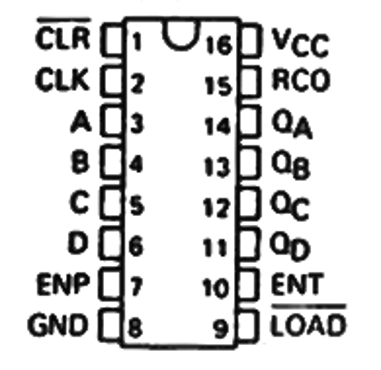
\includegraphics[scale=0.6]{1.png}
                        \label{fig:label}
                    \end{center}

              \item [2.] 同步4比特二进制加法计数器—74LS163                  \\
                    \begin{center}
                        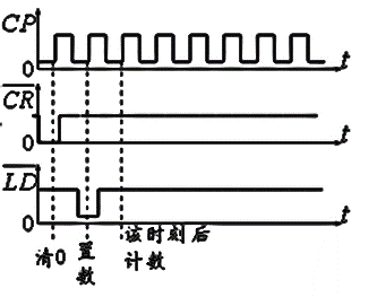
\includegraphics[scale = 0.6]{2.png}
                        \label{fig:label}
                    \end{center}

                    \begin{itemize}
                        \item 同步清零:\overline{CLR}=0+时钟上升沿
                        \item 同步置数:\overline{LD}=0+时钟上升沿
                        \item 模16二进制加法计数:\overline{CLR}=\overline{LD}=1且CT_T=CT_P=1对计数脉冲CP实现同步4比特二进制加法计数
                    \end{itemize}
              \item [3.] 74LS163的应用                  \\
                    实现任意进制的计数和分频的方法\\
                    \begin{itemize}
                        \item 反馈复位法
                        \item 反馈置数法
                        \item 计数器的级联
                    \end{itemize}
                    \begin{center}
                        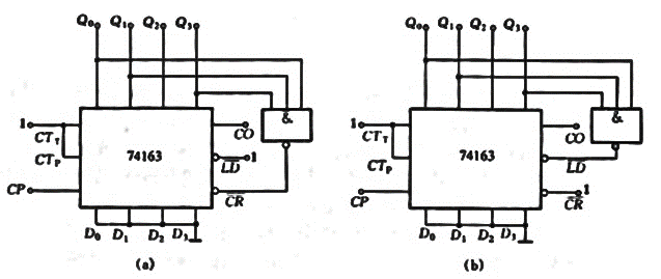
\includegraphics[scale = 0.6]{3.png}
                        \label{fig:label}
                    \end{center}
              \item [4.] 译码器\\
                    计数器将计数值按4比特二进制输出,必须通过译码器把这个二进制数码译成适合于七段数码管显示的编码。\\
                    \begin{center}
                        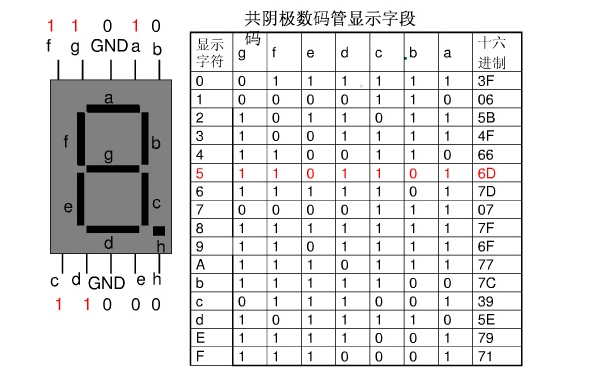
\includegraphics[scale = 0.6]{4.png}
                        \label{fig:label}
                    \end{center}
              \item [5.] CD4511是CMOS BCD-to-7-Segment Latch Decoder Drivers\\
                    \begin{center}
                        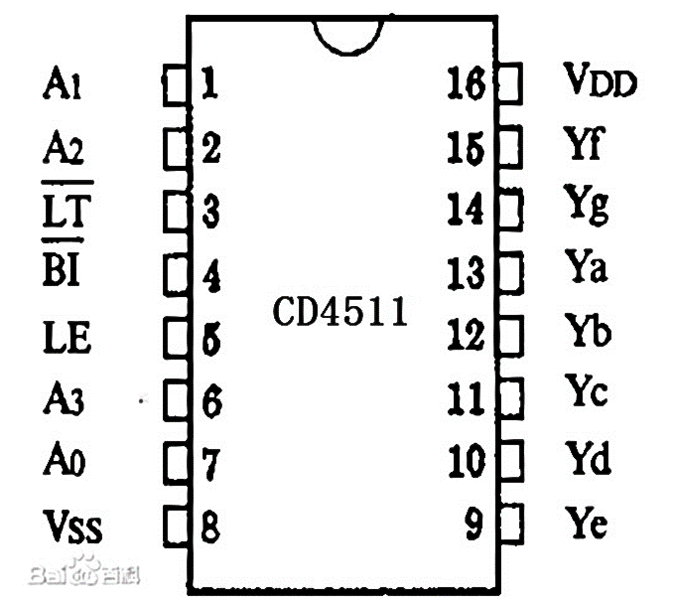
\includegraphics[scale = 0.5]{5.png}
                        \label{fig:label}
                        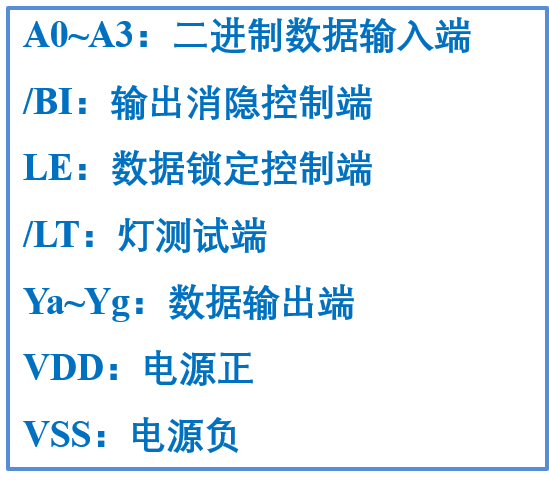
\includegraphics[scale = 0.5]{6.png}
                        \label{fig:label}
                        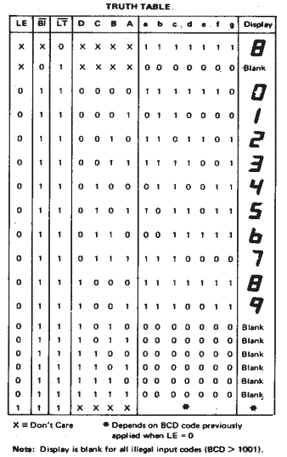
\includegraphics[scale = 0.5]{7.png}
                        \label{fig:label}
                    \end{center}
              \item [6.] 共阴极7段数码管\\
                    数码管是一种半导体发光器件,其基本单元是发光二极管。通过对其不同的管脚输入相对的电压,使其发亮,从而显示出数字,可以用于显示时间、日期、温度等可以用数字表示的参数。在电器特别是家电领域应用极为广泛,如显示屏、空调、热水器、冰箱等等。\\
                    \begin{center}
                        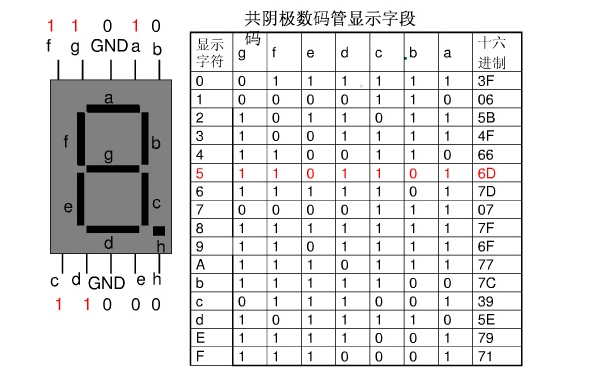
\includegraphics[scale = 0.6]{8.png}
                        \label{fig:label}
                    \end{center}
              \item[7.] 共阴极7段数码管\\
                    \begin{center}
                        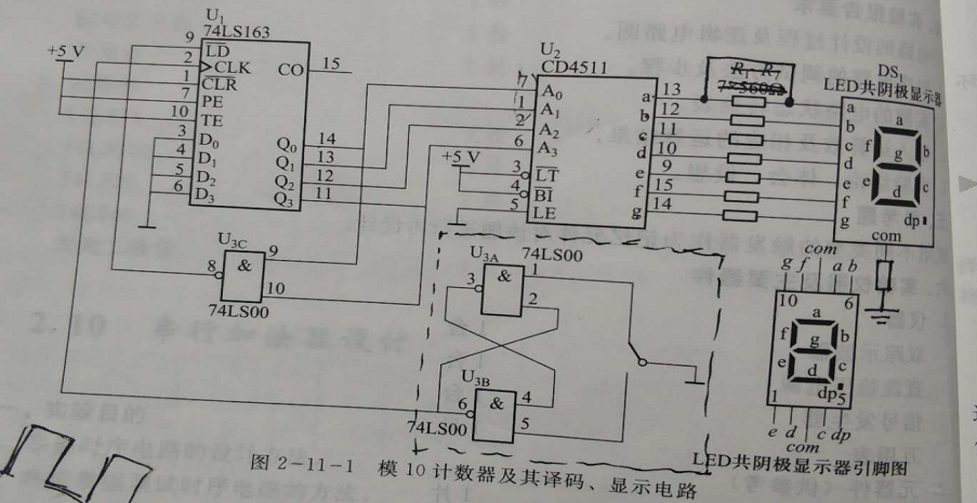
\includegraphics[scale = 0.6]{9.png}
                    \end{center}

          \end{itemize}
    \item 计算及仿真:  \\
          \begin{center}
              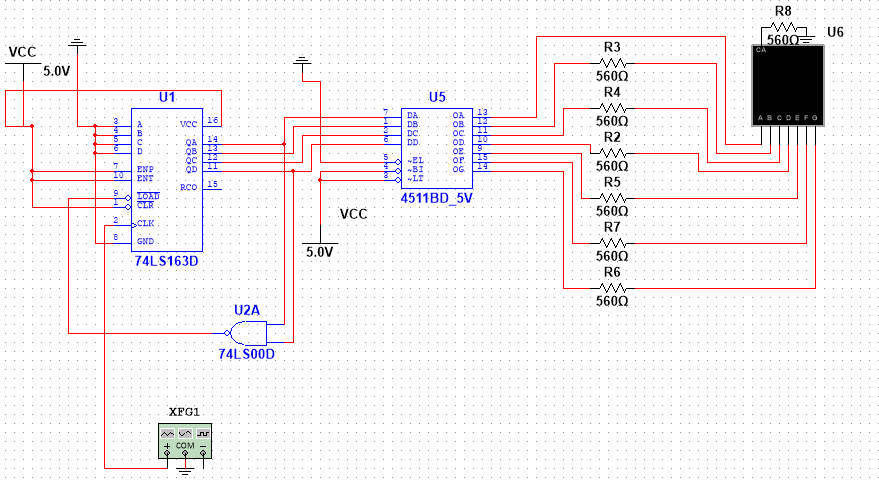
\includegraphics[scale = 0.6]{10.png}
              \label{fig:label}
          \end{center}


    \item  实验目的: \\

          \begin{itemize}
              \item [1.]  掌握中规模集成计数器的基本功能与使用方法
              \item [2.]  掌握中规模集成计数器的变模方法
              \item [3.]  掌握译码器、显示器的工作原理和使用方法。
              \item [4.] 熟悉中规模集成计数器、译码器与显示器互相配合使用的条件和使用方法。
          \end{itemize}
    \item  实验仪器与器件:
          \begin{itemize}
              \item 实验仪器:\\
                    \setlength{\tabcolsep}{30mm}{
                        \begin{tabular}{lr}
                             & 1台 \\
                             & 1台 \\
                             & 1台 \\
                             & 1台 \\
                        \end{tabular}}
              \item 实验器件:\\
                    \setlength{\tabcolsep}{30mm}{
                        \begin{tabular}{lr}
                            74LS163           & 1片 \\
                            CD4511            & 1片 \\
                            74LS00            & 1片 \\
                            7段数码管(共阴) & 1片 \\
                            560欧姆电阻       & 1个 \\
                        \end{tabular}}
          \end{itemize}

    \item  实验过程及数据分析:  \\
          \begin{itemize}
              \item 用74LS163设计一个按照8421BCD码计数的M=10加法器,用7段数码显示器显示计数内容并用示波器观察CP、Q0、Q1、Q2和Q3引脚上的波形。\\
          \end{itemize}
\end{enumerate}
\end{document}